% Chapter 1
\chapter{Introduction} % Main chapter title

\label{Chapter1} % For referencing the chapter elsewhere, use \ref{Chapter1} 

\lhead{Chapter 1. \emph{Introduction}} % This is for the header on each page - perhaps a shortened title

%----------------------------------------------------------------------------------------
Bubbles have fascinated and baffled many canny observers of financial markets. In the language of the strict orthodoxy of the efficient market theory, bubbles are outcome of sudden changes of the fundamental valuation of assets. The empirical evidence denounce that large price jumps can be explained by news, but destabilising feedback loops of behavioural origin \citep{Donier2015}. Although plausible, a clear-cut empirical evidence for
such a scenario is still lacking, but it had created enthusiasms among research communities to understand the origin of bubbles in different commodity, Bitcoin is one of them.

Bitcoin is a digital, distributed, cryptographic currency proposed under the pseudonym Satoshi Nakamoto \citep{Nakamoto2008}. In short, It can be described as a decentralized accounting system in which accounts are associated with public keys of an asymmetric encryption scheme. To access the former account, knowledge of the corresponding private key allows account holders to create digital signatures to send and receive bitcoins (BTC).

\section{Bitcoin Bubble}
\label{sec:bitcoin_bubble}

Bitcoin started trading on Mt.Gox (its market share was over 80\% on the BTC/USD spot market), the largest online Bitcoin exchange at 5 cents. Over the next	 two	 years,	BTC exchange rose slowly, but in early April 2013, the price per BTC dropped from \$266 to around \$50 and then rose to around \$100. This major bubble was succeeded by another one on 29 Nov, 2013, when, the price of a bitcoin reached an all-time high of US\$1224.76, then dropped into the \$200-\$300 range. Metaphorically, the price rise/drop is expressed as skippyball. Once skippyball pitched high in the air, the first bounce is big, then lower, and lower, until it is flat on the ground, ready for a new throw upward. Taking market price data from Blockchain the most popular Bitcoin wallet \footnote{Market Price in USD \url{https://blockchain.info/charts/market-price}}, the bubbles can be visualized in the time series plot \ref{fig:bubble} with circles representing bubbles.

\begin{figure}[ht]
\begin{center}
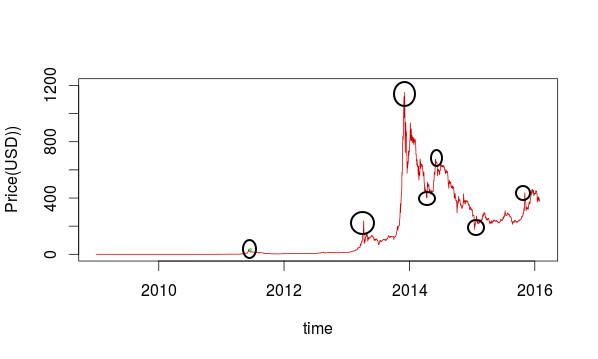
\includegraphics[width=\textwidth]{./Figures/bubble.png}
\caption{BTC Market Price (USD)}
\label{fig:bubble}
\end{center}
\end{figure}

 As the Bitcoin's complete transaction history is stored in an easily accessible and verifiable public ledger called blockchain, It is quite popular amongst economist to study bubbles. The most popular economic explanation \citep{Lo2015, Kristoufek2015} suggests that Bitcoin bubble in April, 2013, was outcome of the financial crisis in Cyprus, which triggered large numbers of people to convert euros into digital BTC. While Bouchaud  and Donier \citep{Donier2015} believe that bubbles were conditioned by the market liquidity, which triggered mismatch between the aggregate market order flow imbalance that becomes strongly negative and the prevailing liquidity on the buy side. In simple words, because of high price, buyers got too scarce to resist the pressure of a sell-off.
 
The complex, cryptic and enormous(over 60 million transactions) data-structure of blockchain had limited researchers to do in-depth transaction analysis even in computer science field. Kondor et al. \citep{Kondor2014} reconstructed the transaction network between users and analyze changes in the structure of the subgraph induced by the most active users. By using unsupervised identification of important features of the time variation of the network and Principal Component Analysis to the matrix constructed from snapshots of the network at different times, they were able to show that structural changes in the network accompany significant changes in the exchange price of bitcoins. The one fall-back about this paper is scalability, which makes it unsuitable for application having nodes greater than 10000 nodes. Other studies \citep{Kristoufek2015} uses digital behavioral traces (eg. twitter etc), wavelet coherence analysis and logistic regression to investigates bubbles, which is not a refine method considering the availability of data \citep{Ali2014}.

\section{Graph Similarity and Subgraph Matching}
\label{sec:gs}
The ultimate goal in financial market is predicting long-term asset prices, as they are so difficult to predict, Bitcoin prices are no different. The margin error with Bitcoin can be particularly brutal for extreme predictions, which usually have a lower probability of being realized. While
there has been significant research done to analyze Bitcoin transaction network, limited research has been executed to analyze the network’s influence on overall Bitcoin price. To achieve the former, one need to efficiently measures the structural change (eg. walks) of a dynamic
large-scale graph as well as the similarity between two graphs with
reference to price change. Kondor et al. \citep{Kondor2014} research was one step in the direction of basic graph similarity and subgraph matching algorithms, which is not scalable with increasing size of daily transactions \ref{fig:transactions}. 

\begin{figure}[ht]
\begin{center}
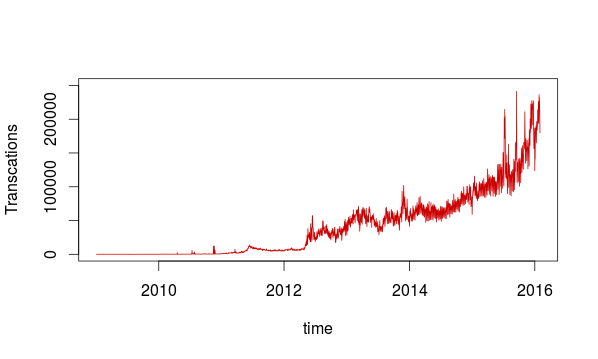
\includegraphics[width=\textwidth]{./Figures/transactions.png}
\caption{Daily Transactions}
\label{fig:transactions}
\end{center}
\end{figure}

Most of graph isomorphism algorithms and its generalizations are exponential and, thus, not applicable to the large graphs that are of interest today. The other methods  for graph similarity and graph sub-matching, like features extractions, iterative methods and tensors analysis, including some come with their drawbacks \citep{Zager2008}.

In the recent paper on graph kernels, Yanardag and Vishwanathan \citep{Yanardag2015} used "Deep Graph Kernels", a unified framework to learn latent representations of sub-structures for graphs to measure similarity. As Bitcoin transaction network graph is increasing everyday, It would be interesting to capture its structural dynamics without compromising on the graph features.

\section{Motivation}
\label{sec: motivation}

The volatile rise and fall of Bitcoin, cryptological mining, complex distributed database, blockchain and evolving network dynamics prompted me to  efficiently measures the structural change (eg. walks) of a dynamic large-scale graph as well as the similarity between two graphs with reference to price change. 

In simple words, the thesis attempts to address two important questions:  
\begin{enumerate}
\item How much is a large-scale graph (bitcoin transaction graph) transformed over time or by a significant event (bubbles)?
\item How structurally similar are two large-scale graph (bitcoin transactions graphs)?
\end{enumerate}

\section{Objective}
\label{sec: objective}

\begin{enumerate}
\item Given complex cryptic distributed blockchain, parsing it to extract transaction attributes in the form transactions graphs.
\item Given two graphs $G_1^{t_1} (n_1 , e_1 )$ and $G_2^{t_2} (n_2 , e_2)$, find an algorithm to calculate the similarity index ($0-1$) between the two graphs. This is quantitative measure of transformation over time.
\item Given a graph time series, where there are $T$ number of graphs, find approximate subgraphs belong to particular events (says bubbles -10-15\% rise/fall in BTC/USD) that occur in a subset of the $T$ graphs. 
\end{enumerate}

\section{Contribution}
\label{sec:contribution}

The decentralized paradigm of Bitcoin requires each node of the network
to retain the blockchain, which consists of all public, transparent, and permanently transactions recorded since the origin. Therefore, blockchain acts as the central point of potentially interesting information ready to be mined. But ever growing size of blockchain (60 GB as of now) makes the job difficult to parse from the raw blockchain. Adding to the same, the newer bitcoin clients indexed the full blockchain using LevelDB makes the earlier public available software obsolete. This thesis aims to develop open source blockchain parsing tools to extract agent resolved data, which can be used to extend the stucked research in bitcoin transaction dynamics. 

To understand how much a large-scale graph (bitcoin transaction graph) transformed over time or by a significant event (bubbles), we use quite novel framework for graph kernels inspired by latest advancements in natural language processing and deep learning, "deep graph propagation kernels" to have quantitative measure of transformation, which captures correlation between network structure and market price. It outperforms its best base variants in terms of capturing .
 

 
\section{Thesis Organization}

The rest of this thesis is organised as follows. In Chapter \ref{Chapter2}, 
we introduces Bitcoin, its working in detail by explaining the protocol of blockchain. Then, the data preparation staged is discussed to get the transaction network, which is used to reproduce transaction dynamics in terms of money flow, also a data validation method.  With data in hand, Chapter \ref{Chapter3} motivates to the graph isomorphism in our context, then reviews the important studies in graph isomorphism problem with advantages and disadvantages. Chapter \ref{Chapter4} starts with review of representative graph kernels in the literature. By taking conventional and sophisticated graph kernels, this chapter defines quantitative measure of transformation over time. The chapter concludes with not so smooth correspondence between network structure and exchange price in bitcoin, thus paving way for further investigation to other graph kernels. With graph kernels not giving desired results, Chapter \ref{Chapter5} propose a general framework that learns hidden representations of sub-structures used in graph kernels, inspired
by deep graph kernels. Then, the framework  is demonstrated on propagation kernels, which performs better than normal kernels. Then new graph kernel is used to calculate similarity index, which is plotted to find correlation between network structure and market price. Chapter \ref{Chapter6} concludes the thesis.

%----------------------------------------------------------------------------------------


